\chapter{Theoretical Foundations}

\section{Linear Algebra in Deep Learning}
Linear algebra forms the cornerstone of deep learning, providing the necessary mathematical framework to model and understand complex relationships within data. It is instrumental in defining the operations and transformations that occur within deep neural networks, including those underlying LLMs.

\subsection{Vectors, Matrices, and Tensors}
Vectors and matrices are fundamental to representing data and parameters in neural networks. A vector $\mathbf{v} \in \mathbb{R}^n$ can represent a point in $n$-dimensional space or a single data instance with $n$ features. Matrices $A \in \mathbb{R}^{m \times n}$ facilitate linear transformations from $\mathbb{R}^n$ to $\mathbb{R}^m$, and tensors generalize these concepts to higher dimensions, accommodating the multi-dimensional data structures processed by neural networks.

A typical case, representing a basic neural network operation, can be expressed as:
\begin{equation}
    \mathbf{y} = A\mathbf{x} + \mathbf{b}
    \label{eq:matrix_multiplication}
\end{equation}
where $A$ is the weight matrix, $\mathbf{x}$ is the input vector, $\mathbf{b}$ is the bias vector, and $\mathbf{y}$ is the output vector of the transformation.

\subsection{Eigenvalues and Eigenvectors}
Eigenvalues and eigenvectors play a critical role in understanding the behavior of linear transformations characteristic of deep learning models. For matrix $A$, if there exists a vector $\mathbf{v} \neq 0$ such that:
\begin{equation}
    A\mathbf{v} = \lambda\mathbf{v}
    \label{eq:eigen}
\end{equation}
then $\lambda$ is called an eigenvalue of $A$, and $\mathbf{v}$ is the corresponding eigenvector. This concept is pivotal in techniques like Principal Component Analysis (PCA), which reduces dimensionality for data visualization and preprocessing.

\subsection{Singular Value Decomposition}
Singular Value Decomposition (SVD) is a powerful technique for decomposing a matrix into singular vectors and singular values, providing insight into the structure of the data. For any matrix $A \in \mathbb{R}^{m \times n}$, SVD is given by:
\begin{equation}
    A = U\Sigma V^T
    \label{eq:svd}
\end{equation}
where $U$ and $V$ are orthogonal matrices containing the left and right singular vectors, respectively, and $\Sigma$ is a diagonal matrix with singular values. SVD is essential in many machine learning tasks, including noise reduction, data compression, and the analysis of neural network layers.

\subsection{Principal Component Analysis (PCA)}
Principal Component Analysis (PCA) is a statistical procedure that uses an orthogonal transformation to convert a set of observations of possibly correlated variables into a set of values of linearly uncorrelated variables called principal components. This transformation is defined in such a way that the first principal component has the largest possible variance (that is, accounts for as much of the variability in the data as possible), and each succeeding component, in turn, has the highest variance possible under the constraint that it is orthogonal to the preceding components. The resulting vectors (principal components) are an uncorrelated orthogonal basis set. PCA is sensitive to the relative scaling of the original variables.

Given a data matrix $X \in \mathbb{R}^{n \times m}$, where $n$ is the number of observations and $m$ is the number of variables, PCA seeks to identify the matrix $W$ that maps $X$ to a new set of variables $Y$, the principal components, such that the variance of $Y$ is maximized. Mathematically, PCA solves for the eigenvalue decomposition of the covariance matrix $X^TX$ or the singular value decomposition (SVD) of $X$ itself.

The covariance matrix $C$ of $X$ is given by:
\begin{equation}
    C = \frac{1}{n-1}X^TX
    \label{eq:covariance_matrix}
\end{equation}
where $X^T$ is the transpose of $X$. The eigenvalue decomposition of $C$ is then performed to find the principal components:
\begin{equation}
    C = W\Lambda W^T
    \label{eq:eigen_decomposition}
\end{equation}
where $W$ is the matrix of eigenvectors (principal components) and $\Lambda$ is the diagonal matrix of eigenvalues (variance explained by each principal component). The columns of $W$ are sorted by decreasing eigenvalues to ensure the principal components are ordered by the amount of variance they explain.

The principal components $Y$ can be obtained by projecting the original data $X$ onto the space defined by the principal components:
\begin{equation}
    Y = XW
    \label{eq:principal_components}
\end{equation}
PCA is widely used in data analysis and for making predictive models. It is commonly used as a tool in exploratory data analysis and for making predictive models. It is also employed to visualize genetic distance and relatedness between populations.

\section{Understanding LLMs}
    Large Language Models (LLMs) such as GPT (Generative Pre-trained Transformer) and BERT (Bidirectional Encoder Representations from Transformers) have revolutionized the field of natural language processing (NLP) by leveraging deep neural networks to understand and generate human-like text unlocking a whole host of new applications.


    \subsection{What are LLMs?}
        LLMs are deep neural networks trained on vast amounts of text data. They learn to predict the next word in a sentence, understand context, generate text, and perform various NLP tasks with minimal task-specific adjustments. The strength of LLMs lies in their ability to capture intricate patterns in language through extensive pre-training.
       
       
        \subsection{Architecture of LLMs}
        The architecture of most LLMs is based on the Transformer model, introduced by Vaswani et al., which relies on self-attention mechanisms to weigh the significance of different words in a sentence. The Transformer architecture is composed of two main components: an encoder and a decoder. The encoder takes the input text and produces a sequence of hidden states, which represent the meaning of the text. The decoder then takes the encoder's hidden states and generates the output text, on word at a time.
            \begin{figure}[h!]
                \centering
                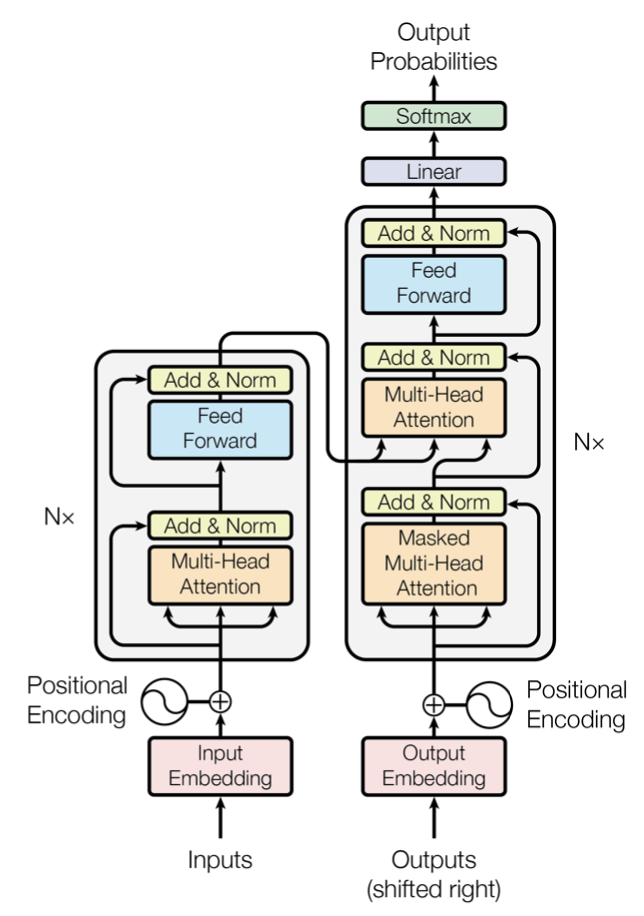
\includegraphics[width=0.5\textwidth]{figs/transform_model.png}
                \caption{Transformer model architecture - Taken from “Attention Is All You Need“}
            \end{figure}
            \subsubsection{Encoder}
            The encoder consists of a stack of \(N\) identical layers, each containing two sub-layers: a multi-head self-attention mechanism and a feed-forward neural network. Furtherly, a residual connection is employed around each of the two sub-layers, followed by layer normalization. So the output of each sub-layer is \(\text{LayerNorm}(x + \text{SubLayer} (x))\), where \(\text{SubLayer}(x)\) represents the function implemented by the sub-layer.
            
            The self-attention mechanism allows the model to weigh the importance of different words in the input sequence when generating the output. The feed-forward neural network processes the output of the self-attention mechanism to produce the final hidden states of the encoder. A key feature of the encoder is that it processes all words in the input sequence in parallel, which contributes to the efficiency of the Transformer model. The output of the encoder is a sequence of vectors, each representing an input word in a high-dimensional space.

            \subsubsection{Decoder}
                The decoder, on the other hand, also consists of a stack of \(N\) identical layers, but with an additional third sublayer in each decoder layer, which performs multi-head attention over the encoder's output. This allows the decoder to focus on different parts of the encoder's output for each word in the output sequence. In the first sublayer of the decoder, self-attention is used, but with a constraint (masking) to prevent positions from attending to subsequent positions. This ensures that the predictions for position \(i\) can depend only on the known outputs at positions less than \(i\). The purpose of the decoder is to generate an output sequence one word at a time, using the encoder's output and what it has produced so far as inputs.

            \subsubsection{Attention}
                The attention mechanism is a crucial component of the Transformer model, allowing it to weigh the importance of different words in the input sequence when generating the output. The attention mechanism is defined as follows:
                \begin{equation}
                    \text{Attention}(Q, K, V) = \text{softmax}\left(\frac{QK^T}{\sqrt{d_k}}\right)V
                    \label{eq:attention}
                \end{equation}
                where $Q$, $K$, and $V$ represent the query, key, and value matrices, respectively, and $d_k$ is the dimension of the key vector. This self-attention mechanism allows the model to focus on relevant parts of the input sequence when performing a task, enabling superior handling of long-range dependencies.
                
            \subsubsection{Multi-head attention}
                Multi-head attention is an extension of the attention mechanism that allows the model to focus on different parts of the input sequence simultaneously. It achieves this by, instead of performing a singel attention function with \(d_{\text{model}}\)-dimensional keys, values and queries, linearly projecting the query, key, and value matrices \(h\) times into multiple subspaces with dimensionality \(d_k\), \(d_k\), and \(d_v\), respectively, before applying the attention function. The output of each of these \(h\) attention heads is then concatenated and linearly projected to produce the final output. This mechanism allows the model to capture different aspects of the input sequence in parallel, enhancing its ability to learn complex patterns in the data.
                \begin{align}
                    \text{MultiHead}(Q, K, V) &= \text{Concat}(\text{head}_1, \ldots, \text{head}_h)W^O \\
                    \text{where head}_i &= \text{Attention}(QW_i^Q, KW_i^K, VW_i^V)
                \end{align}
                Where \(W_i^Q \in \mathbb{R}^{d_{\text{model}} \times d_k}\), \(W_i^K \in \mathbb{R}^{d_{\text{model}} \times d_k}\), \(W_i^V \in \mathbb{R}^{d_{\text{model}} \times d_v}\), and \(W^O \in \mathbb{R}^{hd_v \times d_{\text{model}}}\) are learned linear projections, and \(d_{\text{model}}\) is the dimension of the model.

            \subsubsection{Why Transformers?}
                The Transformer model has several advantages over traditional RNNs and LSTMs, including the ability to capture long-range dependencies, parallelize computation, and scale to larger datasets. The self-attention mechanism allows the model to focus on relevant parts of the input sequence, enabling it to learn complex patterns in the data. The multi-head attention mechanism further enhances the model's ability to capture different aspects of the input sequence in parallel, improving its performance on a wide range of NLP tasks such as translation, summarization, and image captioning. This is why Transformers have become the architecture of choice for many state-of-the-art NLP models, including GPT and BERT.

        \subsection{Training and Fine-Tuning}
            The training of LLMs involves two main phases: pre-training and fine-tuning. During pre-training, the model is exposed to a large corpus of text and learns to predict missing words or sentences, acquiring a broad understanding of language. The fine-tuning phase adjusts the pre-trained model to specific tasks by training on smaller, task-specific datasets. This two-phase approach allows LLMs to achieve remarkable performance across a wide range of NLP tasks with minimal task-specific model modifications.

            \subsection{Training and Fine-Tuning}
            The foundation of an LLM's understanding and generation of human language lies in its pre-training phase. During this stage, the model is exposed to a large corpus of text data, often encompassing a wide range of topics, genres, and styles. The primary objective of pre-training is to enable the model to learn a generalized representation of language.
            
            The pre-training is typically conducted using unsupervised learning techniques, where the model is trained on tasks like Masked Language Modeling (MLM) or Next Sentence Prediction (NSP). In MLM, for example, a percentage of the input tokens are randomly masked, and the model's objective is to predict the original tokens at these masked positions. The MLM objective can be formally represented as:
            
            \begin{equation}
            \mathcal{L}_{\text{MLM}} = -\sum_{i \in \mathcal{M}} \log p(x_i | x_{\backslash \mathcal{M}})
            \end{equation}
            
            where $\mathcal{M}$ is the set of masked positions, $x_i$ is the original token at position $i$, and $x_{\backslash \mathcal{M}}$ represents the input with masked tokens.
            \vspace*{0.2cm}

            Following pre-training, LLMs undergo a fine-tuning phase, wherein the model is specialized to perform specific NLP tasks. This phase involves training the pre-trained model on a smaller, task-specific dataset, allowing the model to adjust its weights to better perform the target task.
            
            The fine-tuning process can be represented as a continuation of the training process, optimizing the following objective:
            
            \begin{equation}
            \mathcal{L}_{\text{fine-tune}} = -\sum_{(x,y) \in \mathcal{D}_{\text{task}}} \log p(y | x; \theta_{\text{pre-train}} + \Delta\theta)
            \end{equation}
            
            where $\mathcal{D}_{\text{task}}$ is the task-specific dataset, $(x,y)$ are the input-output pairs, $\theta_{\text{pre-train}}$ are the parameters learned during pre-training, and $\Delta\theta$ represents the parameter updates during fine-tuning.
            \vspace*{0.2cm}

            Fine-tuning LLMs presents challenges such as catastrophic forgetting and overfitting, particularly when the task-specific dataset is small. Various strategies, including careful learning rate selection, regularization techniques, and the use of adapters, are employed to mitigate these issues.
            